
\subsection{Runtime}
The ZOne runtime is primarily written in C/C++. The ZOne runtime provides all
normal language runtime functions with a focus on hiding I/O latency. The ZOne
compiler provides information to the runtime about what tasks can be
interleaved. These runtime features are built on top of CUDA streams and 
Intel Threaded Building Blocks. The following sections describe the
implementation of the ZOne runtime.
We have included the code for Black-Scholes in the appendix in listing~\ref{lst:blackscholes} as an example code of how one writes code using our runtime.

\subsubsection{Overview}


\begin{figure}
\centering
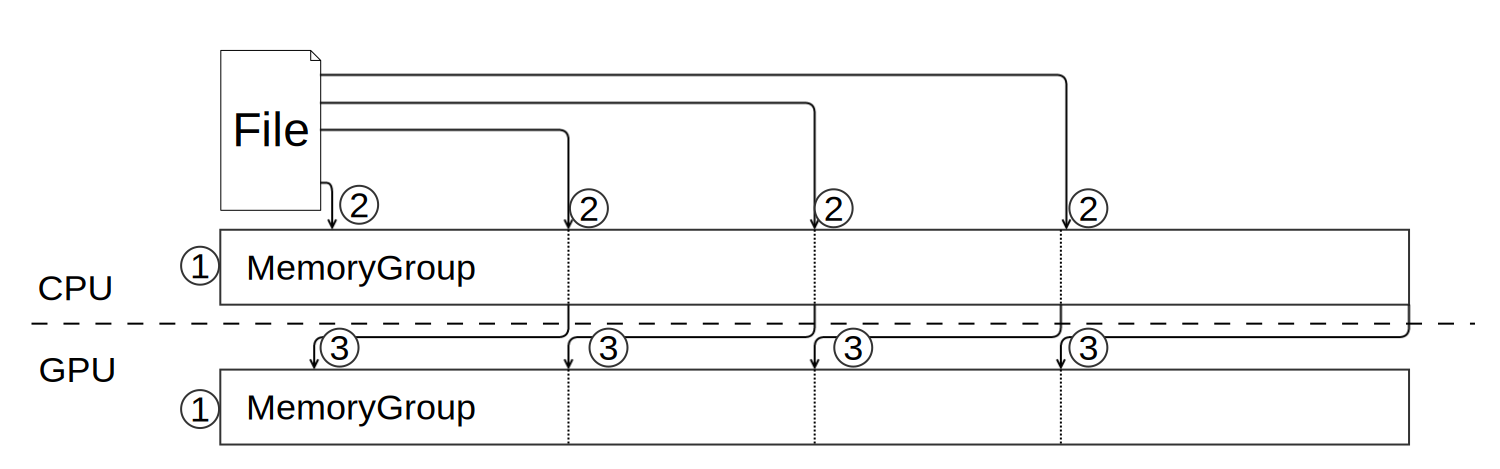
\includegraphics[scale=0.2]{fig/memory_group.pdf}
\caption{Memory Streaming Design}
\label{fig:memorygroup}
\centering
\end{figure}

The purpose of the runtime is two fold.
First, it simplifies our code generation --- alowing us to 
	have a unified view of memory and simplifying the 
	code generator.
Second, it eagerly copies data to the GPU.

The runtime does a few things to solve these problems.
To unify memory, we create a new object called \fix{zMemoryGroup\_t}
	this object contains multiple \fix{zMemory\_t} which 
	index into a contiguious array buffer for both CPU and GPU memories.
Each \fix{zMemory\_t} holds a state, such as
	\fix{unalloacted}, \fix{allocated},
	\fix{dirtyDevice}, etc\ldots
	that allow us to maintain conherence and avoid copies when
	not necessary.
The memory object also contain size and type information,
	and we operate on \fix{zMemory\_t} rather than a \fix{void *}
	types.
The abstract also facilitates us to other language supports, such 
	as OpenCL, without changing our code generator.

To eagerly copy memory to the GPU, we use logic similar to what is
	shown in figure~\ref{fig:memorygroup}.
In (1), we concurrently alloate CPU memory and GPU memory.
The file is then opened in (2) and different chunks are read into
	the CPU memory one it's been allocated (we \fix{mmap} the file
	with the \fix{PROT\_READ, MAP\_PRIVATE} options to increase
	performance).
Once a chunk of data is read, and GPU memory is allocate, data 
	is copied to the GPU in (3).
Note that while we have independent view of chunks of memory 
	(defined by the datatype \fix{zMemory\_t}) memory is in fact
	contiguious and placed in a \fix{zMemoryGroup\_t} object.
This makes it possible to free memory efficiently, and, althought
	not presently implemented, allows us to resize the chunk
	sizes.


\subsubsection{Intel Threaded Building Blocks}
Intel Threaded Building Blocks \cite{reinders2007intel} (TBB) is a library for
scalable parallel
programming in C++. It provides templates for common parallel programming
patterns and abstracts away the details of synchronization, load-balancing,
and cache optimization. Instead of writing threads the programmer specifies
tasks, and the library maps them onto threads in an efficient manner.

\subsubsection{CUDA Streams}
By design, CUDA device kernels execute asycnhronously with respect to the
host code. This allows host code to overlap with device code, but does not
allow different device operations (kernels and data transfers) to execute
concurrently. CUDA exposes device concurrency through \textit{CUDA Streams}
\cite{kirk2012programming}.

A CUDA Stream is a sequence of operations that
execute in-order on a CUDA device. Separate streams may be interleaved or
overlap if possible. In this way, it is possible to overlap computation and
memory transfers to hide the latency of some operations.
In order to effectively use streams, CUDA allows synchronization operations
to occur between arbitrary streams and provides host code that allows the
CPU to determine the execution status and progress of different streams.

The flexibility of CUDA streams is limited by the device hardware.
For example, the Fermi architecture can manage one queue of kernels, one queue
of device$\rightarrow$host transfers, and one queue of host$\rightarrow$device
transfers. Stream
dependencies between queues are maintained, but there are no dependencies
within queues - the operations are simply done in the order they are put into
the queue.
On devices that support more than one concurrent compute operation the amount
of concurrency is limited by the execution resources on the device. If both
operations are too large to run concurrently they will be serialized.


CUDA streams are used for our copy operations and we register callbacks via the \fix{cudaStreamAddCallback} function to set flags and clear mutexes once
the asynchronus requrest completes.
These flags and mutexes are checked before a kernel launch or copy to either	make sure the data is available before a computation, or that data has
	already been copied and does not need to be recopied.

	


\subsubsection{Limitations}

One of the main limitations of the runtime is that the sizes of files need to
	be known beforehand.
This is because we start allocating memory before a file is open.
A slight modification to the runtime would allow us to read file meta data 
	before starting to allocate.

Another limitation is that files are assumed to be encoded as a raw byte
	array of a specific C type.
This avoids us having to write logic to parse the file.

Both of these limitations manifest themselves because we did not want to 
	write a generic file format or file importer, since this is a problem 
	orthogonal to this project.
In the future, one can use file formats,
	such as HDF~\cite{folk2011overview}, to circumvent these implementation
	limitations.

In the case of requiring one to parse a file to extract its data into
	C datatypes, we expect that we would see more performance
	improvement, since we can perform this parsing in parallel.